% Small intro, re-explain that finding thread/core pairing is complicated and thus ML is a good idea.
As seen in the previous section, selecting the right number of threads and a good combination of cores is difficult.
This difficulty arises from trying to balance between exploiting larger composed cores with block speculation and ILP and between exploiting a larger number of logical cores via TLP.

The problem can be decomposed into two stages; first, determining the right number of threads and then selecting a good core composition.
In this section, two machine-learning models that predict the best thread partitioning and core composition to maximize performance are presented.

\subsection{Predicting the Best Number of Threads}

\paragraph{Synthetic Benchmark Generation}

One of the difficulties of building a machine learning based model for StreamIt is the lack of benchmarks available~\cite{wang2013partitionstreamit}.
Whilst there exists at least 30 realistic applications for StreamIt~\cite{theis2010empericalcharstreamit} this is simply not enough to create a large enough data set.
To overcome this problem synthetic StreamIt benchmarks are generated and gather statistics from them in a similar style as in~\cite{wang2013partitionstreamit}.
To ensure that the synthetic benchmarks are representative of realistic benchmarks they are created using filters from a set of micro-kernels found in some StreamIt examples.
30 different possible filters with different incoming and outgoing rates, different inputs and outputs are used.
To ensure that the synthetic benchmarks were similar to real benchmarks, the total number of filters and split joins are within the average of the realistic benchmarks.

For each generated application, 15 different threaded versions are generated.
Each of these versions is ran using a single core per thread and the cycle count is recorded.
This was repeated for 1000 unique randomly generated applications and record the best number of threads each time.

\paragraph{Extracting Features}

Once the benchmarks have been generated, the next step consists of gathering features for each applications.
In order to build the two machine learning models an initial set of over 50 features are extracted from StreamIt programs.
These features were extracted using pre-existing tools within StreamIt and some extra counters added by us.
The features selected for the models were determine through correlation analysis.
%In this section, when discussing correlation we specifically look at which variables correlate with the optimal number of threads.
In this section, variables which correlate with the optimal number of threads are explored.
These features are used by the model to make a prediction about the number of threads to use.

Figure~\ref{fig:corr} shows the 10 variables that correlate the most with the optimal thread number.
In StreamIt the term multiplicity references the number of times a filter will have to execute in a time slice when the graph is in a steady state~\cite{gordon2002streamcomp}.
In Figure~\ref{fig:corr} the highest correlating value, Number of Distinct Multiplicities, determines all different multiplicities found in the StreamIt graph.
Unconditionally executed blocks represent sets of operations in a filter that will always execute.

There are very little variables that highly correlate beyond Number of Distinct Multiplicities.
A high number of distinct multiplicities implies that subsets of filters will execute at different rates.
This means that certain filters may be local bottlenecks in a Pipeline for example.
When the number of distinct multiplicities is high this requires more threads to group filters with similar multiplicities.
The number of threads also depends on certain structural features such as Pipelines, SplitJoins and number of Filters.
Yet, these variables seem to hold less influence on the number of threads a program needs than the different multiplicities found in the graph.
This is most certainly due to the fact that whilst SplitJoins make parallelizable areas more visible, the amount of work contained in each stream of the SplitJoin, especially when this size is small, may actually make parallelizing the program worse due to ratio of communication to computation.

\begin{figure}
  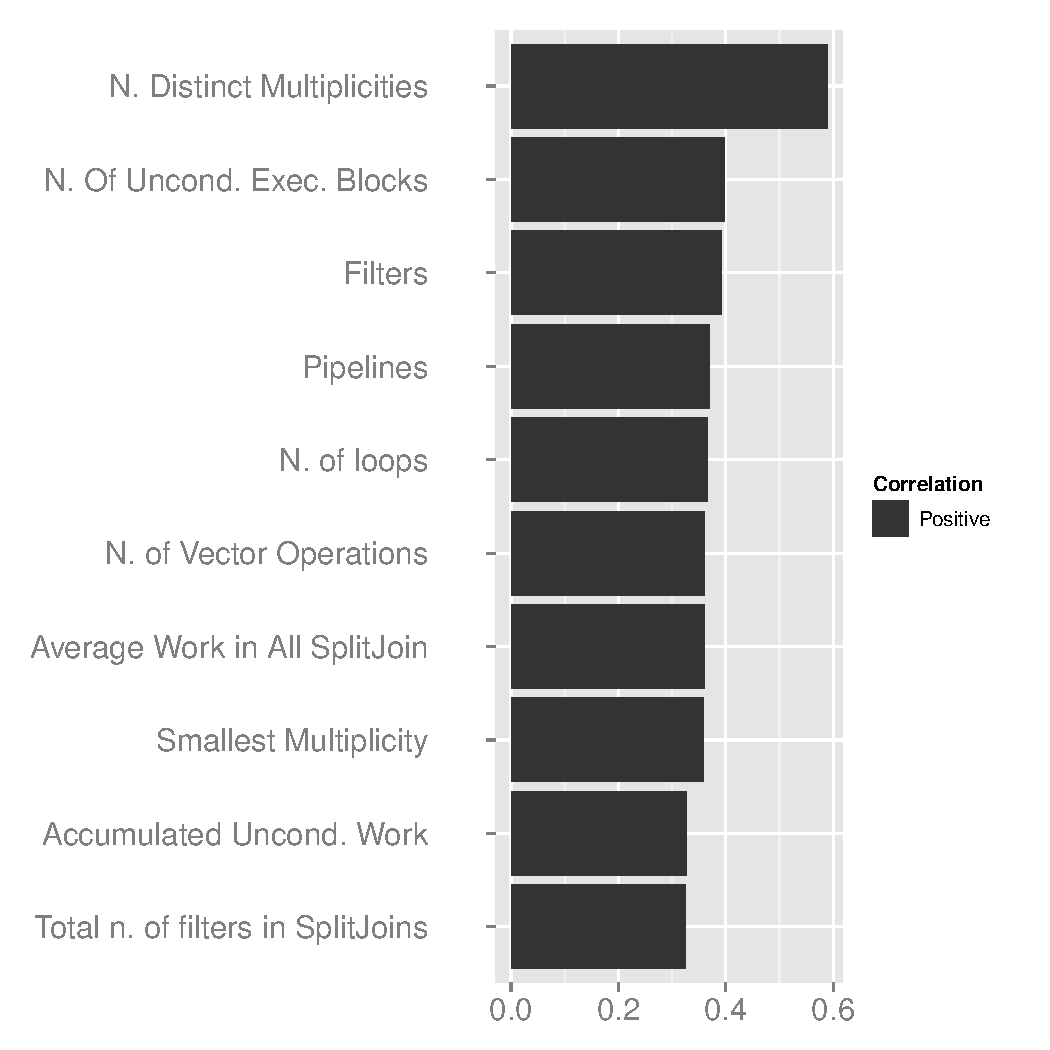
\includegraphics[width=1\textwidth]{streamit-paper/graphics/corrGraph.pdf}
  \caption{The ten highest correlating features with the best number of threads for 1000 synthetic benchmarks.}\label{fig:corr}
\end{figure}
 
\paragraph{KNN Model}

A k-Nearest Neighbor (kNN) model was chosen to determine the number of threads to use for the application.
Given a new application to predict, the kNN classifier determines the $k$ closest generated applications in terms of the features.
The distance between the features is measured using the Euclidean for each application.
Once the set of $k$ nearest neighbors has been identified, the model simply averages the best number of threads for each of the $k$ nearest neighbors to make a prediction.
The parameter $k$ was determined experimentally using only the generated benchmarks.
A value of $k=7$ was found to lead to the best performance.

The features chosen are the variables displayed in Figure~\ref{fig:corr}.
Using cross validation is used to determine the efficiency by observing how close a classification is to the measured best thread number.
Using cross validation the model generated in this chapter has a 33\% accuracy of getting the predicted best thread number.
This increases to 57\% when allowing a prediction to be 1 thread away from the best and 67\% when 2 threads away.
Whilst the performance of pin-point accuracy is disappointing it does not incur more than a 12\% performance penalty when choosing a thread number which is +/- 1 from the best and 19\% when moving up to 2 threads away from the best.
This average is measured by looking at the thread performances without composition.

\begin{figure*}
  \center
  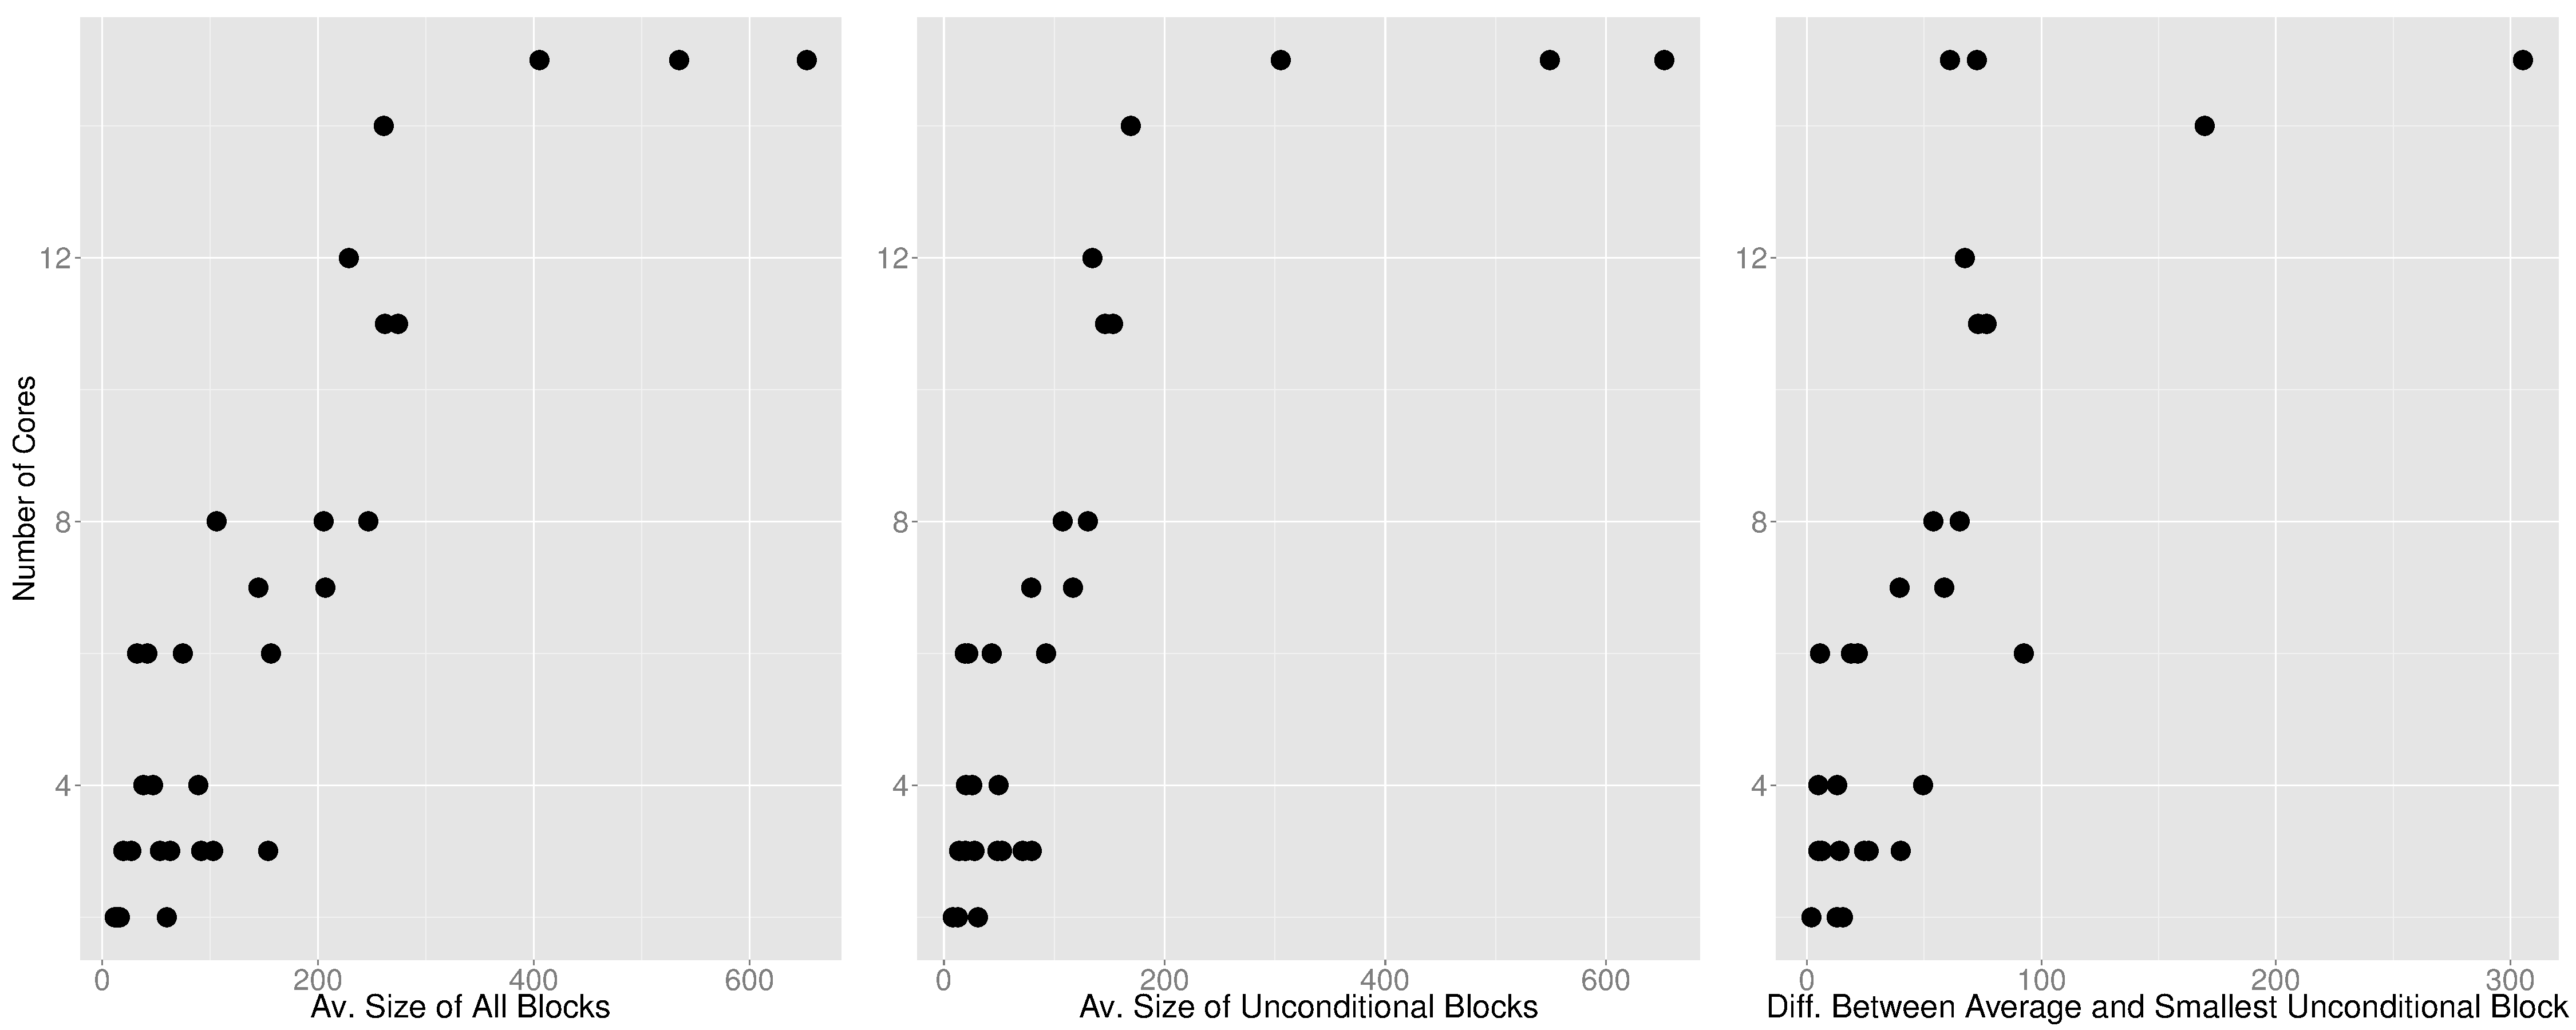
\includegraphics[width=1\textwidth]{streamit-paper/graphics/lineargraphs.pdf}
  \caption{Optimal number of cores in relation to the three highest correlating features. The maximum number of cores plateaus on the right hand side as this is the maximum possible amount.}\label{fig:maxav}
\end{figure*}
